% Created 2022-10-10 Mon 10:15
% Intended LaTeX compiler: pdflatex
\documentclass[11pt]{article}
\usepackage[utf8]{inputenc}
\usepackage[T1]{fontenc}
\usepackage{graphicx}
\usepackage{grffile}
\usepackage{longtable}
\usepackage{wrapfig}
\usepackage{rotating}
\usepackage[normalem]{ulem}
\usepackage{amsmath}
\usepackage{textcomp}
\usepackage{amssymb}
\usepackage{capt-of}
\usepackage{hyperref}
\usepackage{parskip}
\author{Omkar Girish Kamath}
\date{\today}
\title{Specification Document}
\hypersetup{
 pdfauthor={Omkar Girish Kamath},
 pdftitle={Specification Document},
 pdfkeywords={},
 pdfsubject={},
 pdfcreator={Emacs 26.3 (Org mode 9.1.9)}, 
 pdflang={English}}
\begin{document}

\maketitle
\tableofcontents

\section{Instruction set of the processor}
\label{sec:org0bd2aa9}

In this instruction syntax X=Not used, K=Constant, A=Instruction Address, P=Data Address

\textbf{Load} ACC kk : 0000 XXXX KKKKKKKK

\textbf{Add} ACC kk : 0100 XXXX KKKKKKKK

\textbf{And} ACC kk : 0001 XXXX KKKKKKKK

\textbf{Sub} ACC kk : 0110 XXXX KKKKKKKK

\textbf{Input} ACC pp : 1010 XXXX PPPPPPPP

\textbf{Output} ACC pp : 1110 XXXX PPPPPPPP

\textbf{Jump} U aa : 1000 XXXX AAAAAAAA

\textbf{Jump} Z aa : 1001 00XX AAAAAAAA

\textbf{Jump} C aa : 1001 10XX AAAAAAAA

\textbf{Jump} NZ aa : 1001 01XX AAAAAAAA

\textbf{Jump} NC aa : 1001 11XX AAAAAAAA

The register transfer level (RTL) description of each of these instructions is:

Load ACC kk : ACC <- KK

Add ACC kk : ACC <- ACC + KK

And ACC kk : ACC <- ACC \& KK

Sub ACC kk : ACC <- ACC - KK

Input ACC pp : ACC <- M[PP]

Output ACC pp : M[PP] <- ACC

Jump U aa : PC <- AA

Jump Z aa : IF Z=1 PC <- AA ELSE PC <- PC + 1

Jump C aa : IF C=1 PC <- AA ELSE PC <- PC + 1

Jump NZ aa : IF Z=0 PC <- AA ELSE PC <- PC + 1

Jump NC aa : IF C=0 PC <- AA ELSE PC <- PC + 1

Here '->' indicates updated with .
\section{Modules in the processor}
\label{sec:orgf06bb92}
\subsection{RAM}
\label{sec:org9ca0800}
\subsubsection{Theory}
\label{sec:org2546f1f}
\subsubsection{Interface}
\label{sec:org2329f18}
\subsection{Program Counter}
\label{sec:orgd901d66}
\subsubsection{Theory}
\label{sec:orga91ccac}
\begin{figure}[htbp]
\centering
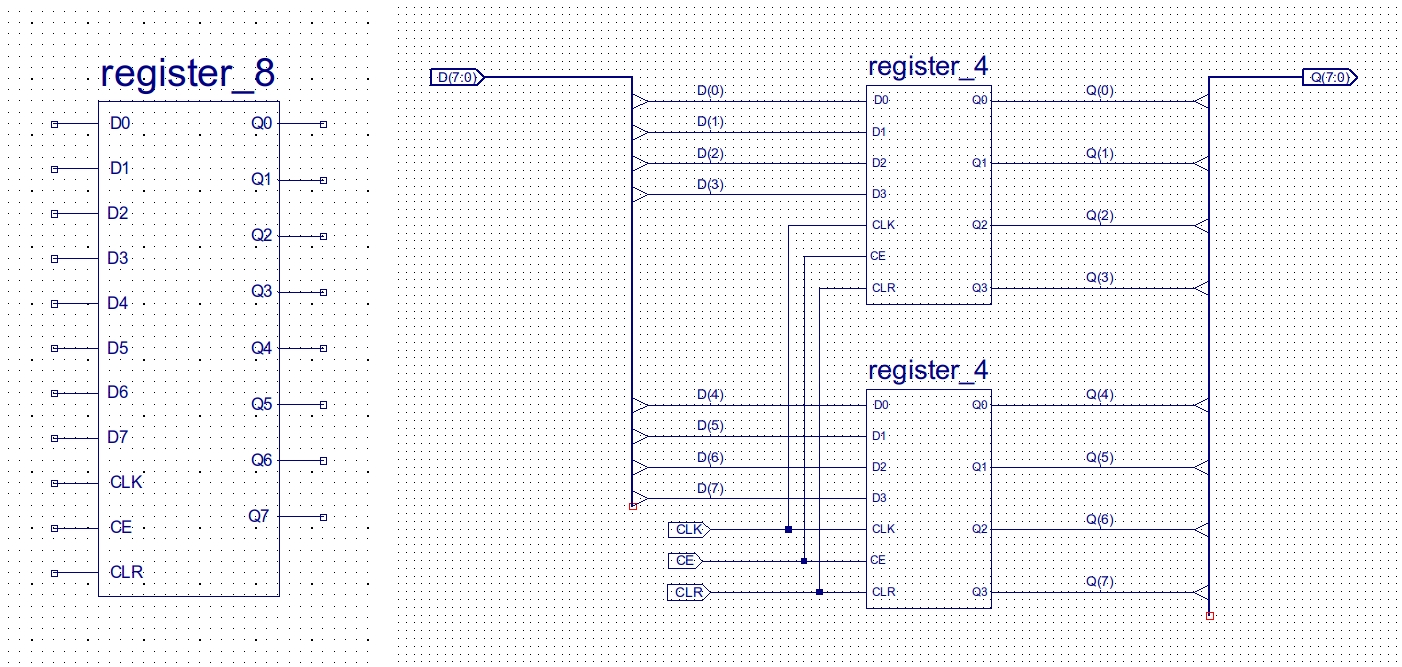
\includegraphics[width=.9\linewidth]{./images/reg8.jpg}
\caption{\label{fig:org44c72d1}
}
\end{figure}
8 bit register used to store the address \textbf{current} instruction being executed.
It is incremented after every \emph{fetch-decode-execute-increment} cycle .
\subsubsection{Interface}
\label{sec:orgbe15afa}
module pc (\\
d,\\
clk,\\
ce,\\
clr,\\
q\\
);

input [7:0] d     ; \\
input clk         ;   \\
input ce      ; \\
input clr     ; \\
output [7:0 ]q; \\

\begin{center}
\begin{tabular}{lll}
signal name & type & size\\
\hline
d & input & 8 bits\\
clk & input & 1 bit\\
ce & input & 1 bit\\
clr & input & 1 bit\\
q & output & 8 bits\\
 &  & \\
\hline
\end{tabular}
\end{center}
\subsection{Instruction Register}
\label{sec:org6eebe5e}
\subsubsection{Theory}
\label{sec:orga413288}
Instruction Register (IR) : \textbf{16} bit register, updated at the end of the fetch phase with the instruction to be processed (decoded and executed).
\begin{center}
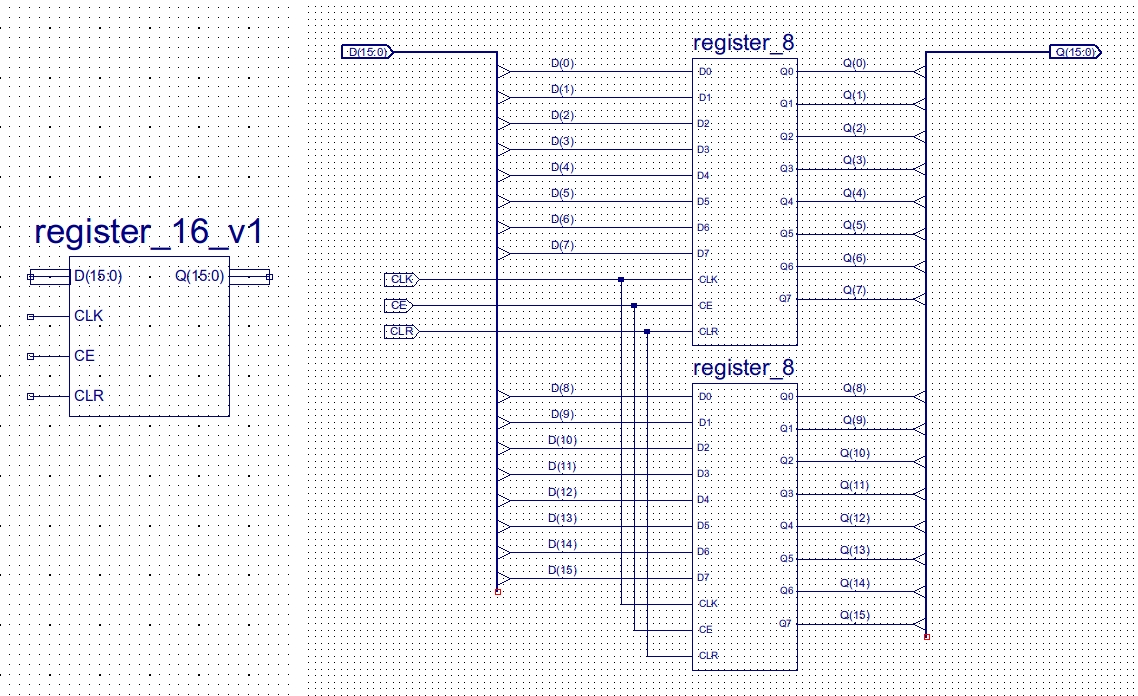
\includegraphics[width=.9\linewidth]{./images/reg16.jpg}
\end{center}
\subsubsection{Interface}
\label{sec:org5a0166f}
module ir (\\
    d,\\
    clk,\\
    ce,\\
    clr,\\
    q\\
    );\\

input  [15:0] d     ; \\
input         clk   ;   \\
input         ce    ; \\
input         clr   ; \\
output [15:0] q     ; \\

\begin{center}
\begin{tabular}{lll}
signal name & type & size\\
\hline
d & input & 16 bits\\
clk & input & 1 bit\\
ce & input & 1 bit\\
clr & input & 1 bit\\
q & output & 16 bits\\
\hline
\end{tabular}
\end{center}

\subsection{Decoder}
\label{sec:orged2420a}
\subsubsection{Theory}
\label{sec:org9283c64}
It generates the sequence of control signals needed to perform the functions defined by each instruction by considering the current state of the processor and the current instruction . These are contained within the decoder or control-logic block , the circuit diagram symbol for this component is shown.
\begin{center}
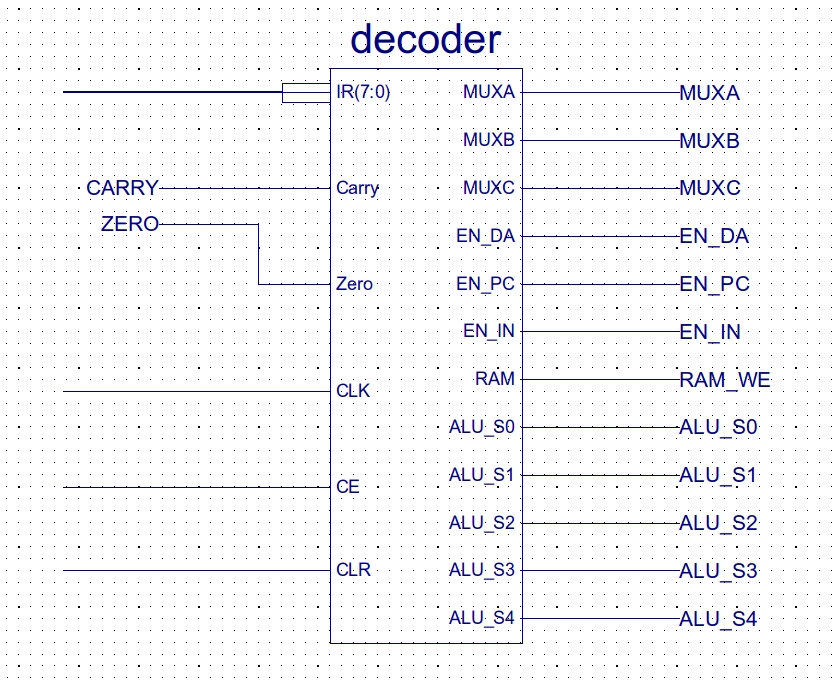
\includegraphics[width=.9\linewidth]{./images/decoder_sym.jpg}
\end{center}

The different parts of the decoder is shown in the figure given
\begin{center}
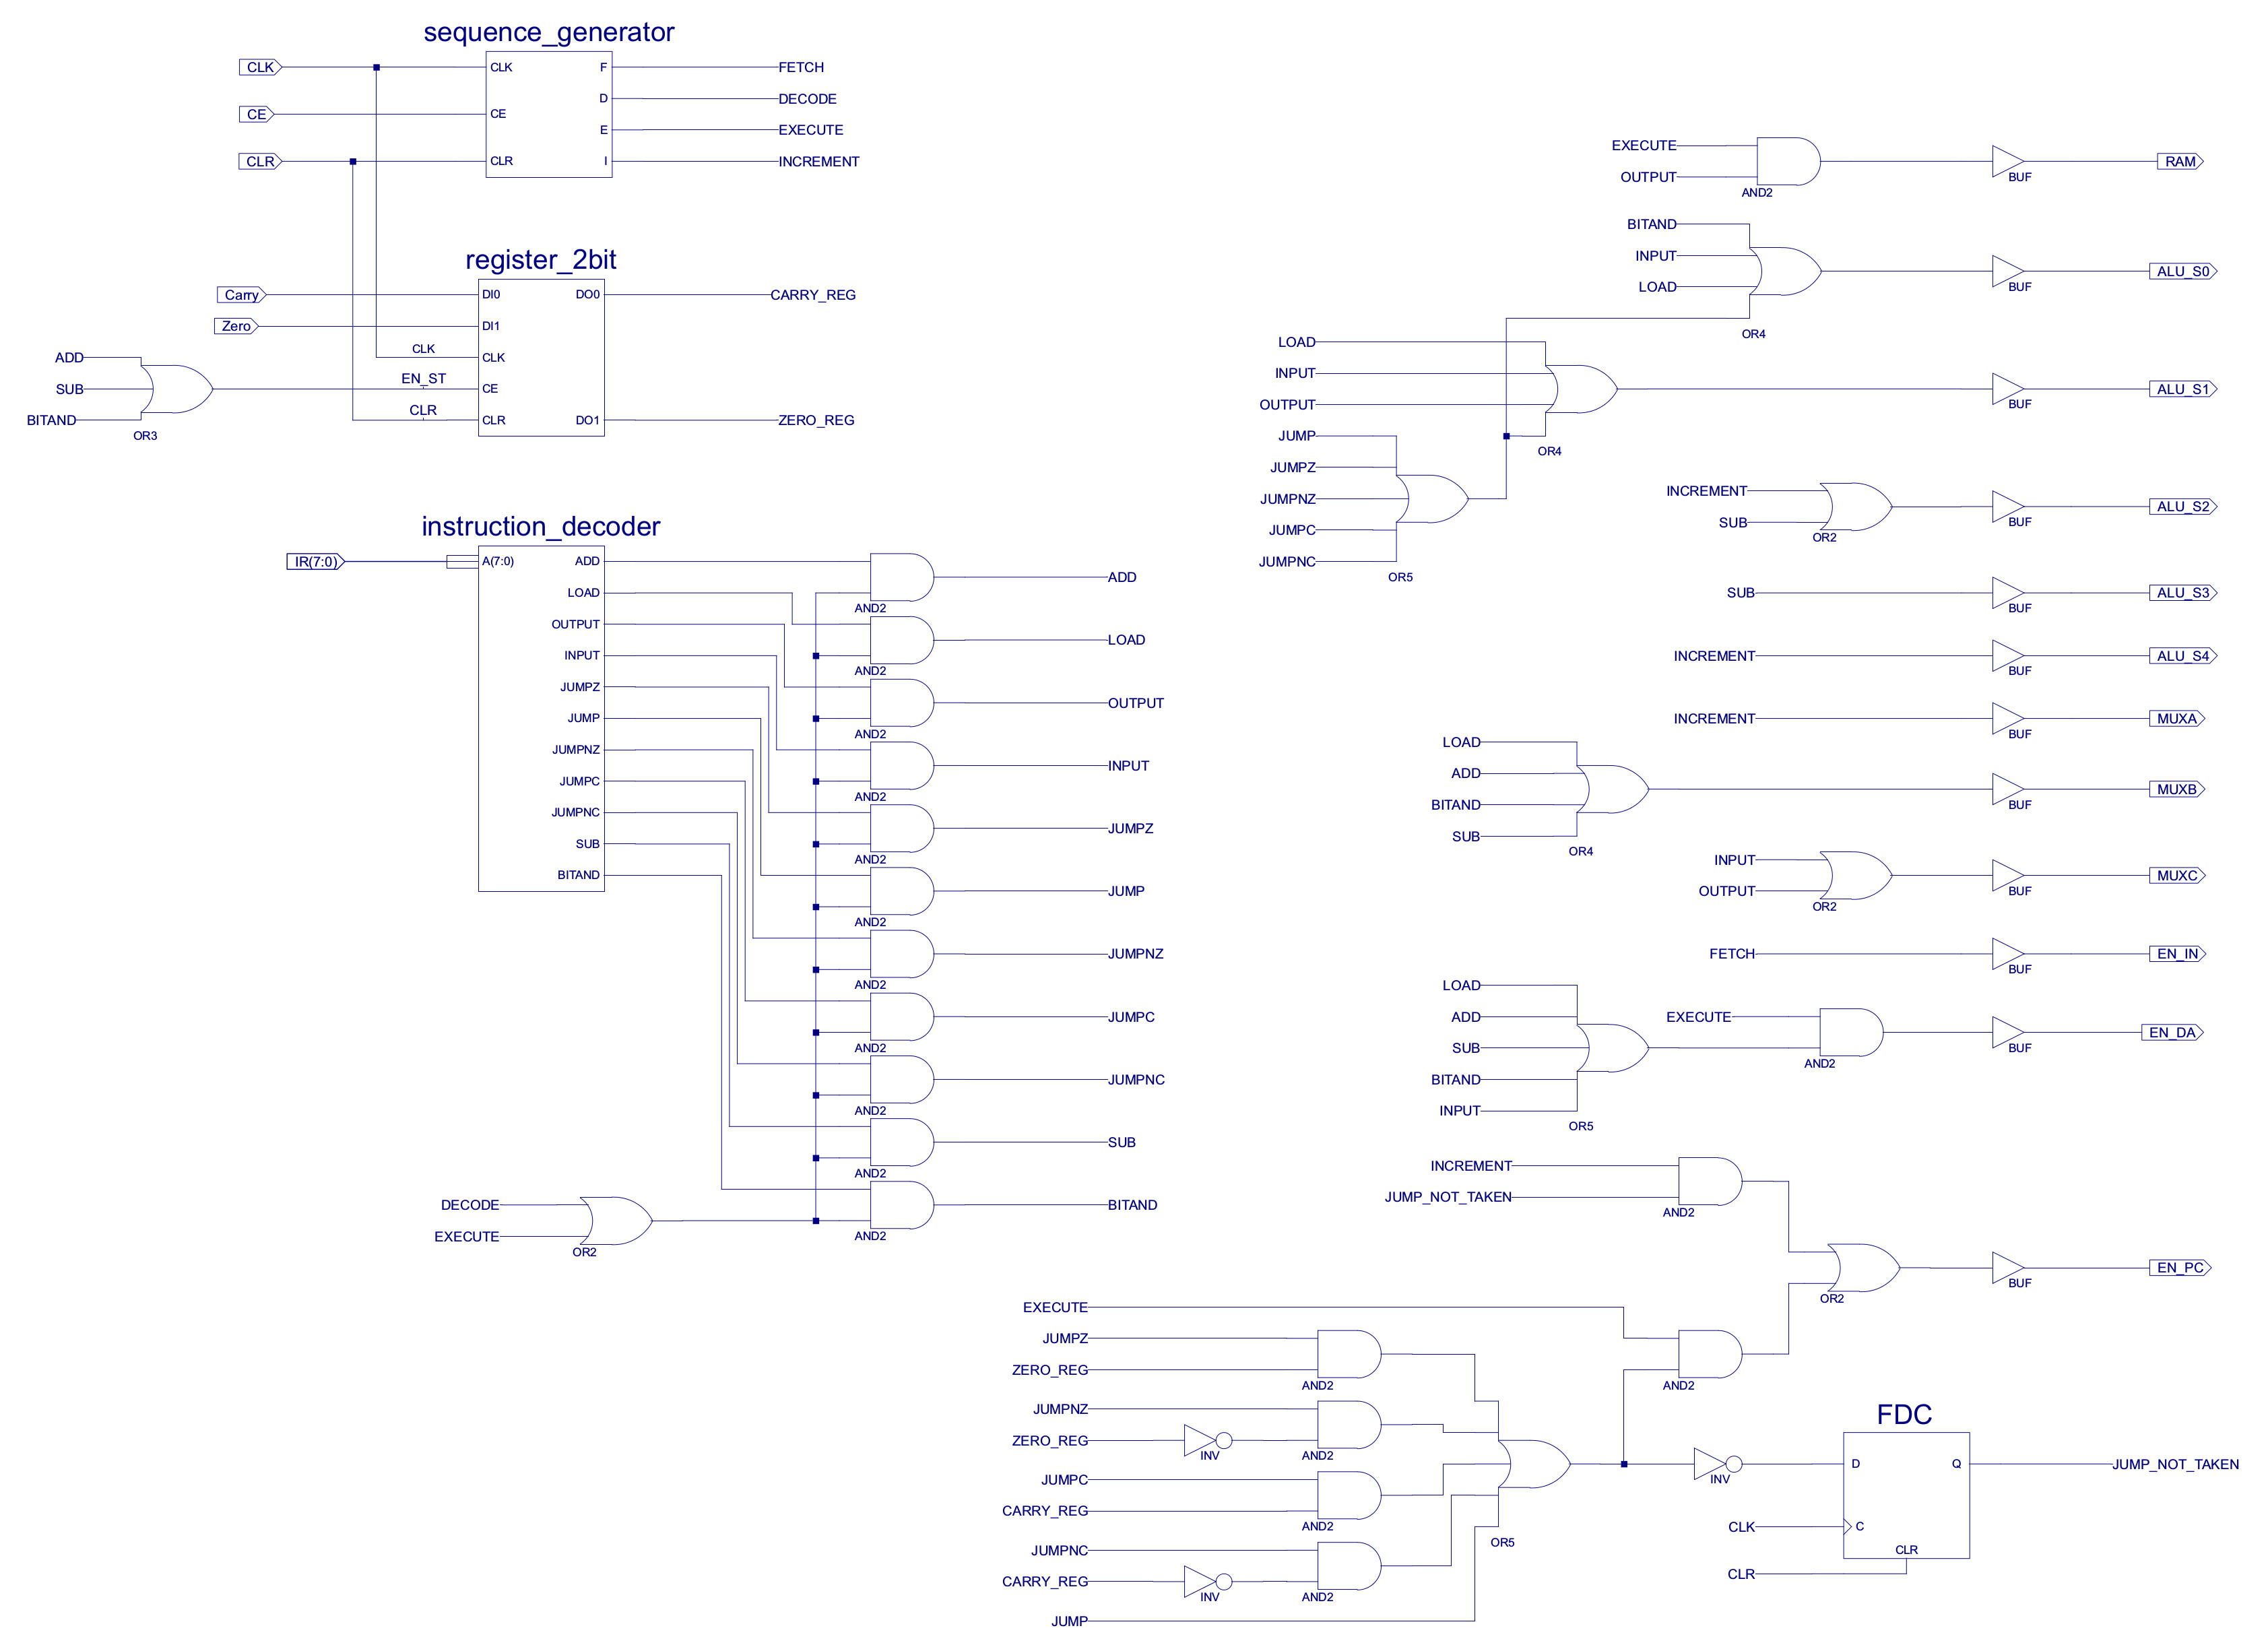
\includegraphics[width=.9\linewidth]{./images/decoder.jpg}
\end{center}


\textbf{(a)} \uline{SEQUENCE GENERATOR}

To identify which phase the processor is in a sequence generator is used , This is a simple ring counter , using a one-hot (Link) encoded value to indicate the processor's state .
Initially the value 1000 is loaded into the counter (fetch code), on each clock pulse the one-hot bit is then moved along the flip-flop chain, looping back to the start after four clock cycles. To determine the processor's state you simply identify which bit position is set to a logic 1. One-hot encoding i.e. when a number only ever has one bit set, is very easy to decode in hardware, but its sparse encoding means you need a lot of bits to represent larger values as not all bit states are used. A four bit one-hot value can represent 4 states, or the value 0 to 3, using a binary encoding you could represent the value 0 to 15, but you would need to decode all bits to determine its value, where as using one-hot you only need to look at one bit.

1000 : Fetch

0100 : Decode

0010 : Execute

0001 : Increment

\textbf{(b)} \uline{INSTRUCTION DECODER}

The top 4 to 6 bits of each instruction defines the opcode: an unique binary pattern that allows the CPU to identify what function needs to be performed, where the data (operands) are and where any result produced should be stored. Note, the top nibble (4bit) of each instruction is unique to that instruction. The instruction decoder  converts the unique opcode into a one-hot value, these are then used during the Decode and Execute phases to control the processor's hardware. To ensure these signals are not active during the Fetch and Increment phases they are ANDed (zeroed) with the result of the logical OR of the Decode and Execute signals from the sequence generator. \\


Most of this control logic is quite intuitive, you simply combine the one-hot output from the Decoder with the state bits from the Ring-counter to produce the logic 1's in each row of the table in figure 32 . A slightly more complex bit is the Jump logic . If the processor is in the Execute phase, the instruction decoder and status signals determine if the program counter (PC) should be updated i.e. should the jump address be loaded into the PC. If a JUMP instruction is taken, then the system does not need to increment the PC, as it already contains the address of the next instruction. Therefore, when the processor is in the Increment phase it checks to see if a jump has been taken, if it has been the PC is not enabled i.e. the result PC+1 is not stored in the program counter.




\subsubsection{Interface}
\label{sec:org4082eaf}
\begin{center}
\begin{tabular}{lrll}
Name & size & function & type\\
\hline
mux\(_{\text{a}}\) & 1 & ALU A input MUX control & output\\
mux\(_{\text{b}}\) & 1 & ALU B input MUX control & output\\
mux\(_{\text{c}}\) & 1 & address MUX control, selecting PC or IR & output\\
en\(_{\text{da}}\) & 1 & accumulator (ACC) register update control & output\\
en\(_{\text{pc}}\) & 1 & program counter (PC) register update control & output\\
en\(_{\text{ir}}\) & 1 & instruction register (IR) update control & output\\
ram\(_{\text{we}}\) & 1 & memory write enable control & output\\
alu\(_{\text{c}}\) & 5 & ALU control line & output\\
ir & 8 & high byte of instruction register, contains opcode & input\\
zero & 1 & connected to ALU output, if 1 indicates result is zero & output\\
clk & 1 & system clock & input\\
ce & 1 & clock enable, normally set to 1, if set to 0 processor will HALT & input\\
clr & 1 & system reset, if pulsed high system will be reset & input\\
\hline
\end{tabular}
\end{center}


MUX\(_{\text{A}}\) : output, ALU A input MUX control

MUX\(_{\text{B}}\) : output, ALU B input MUX control 

MUX\(_{\text{C}}\) : output, address MUX control, selecting PC or IR 

EN\(_{\text{DA}}\) : output, accumulator (ACC) register update control 

EN\(_{\text{PC}}\) : output, program counter (PC) register update control 

EN\(_{\text{IR}}\) : output, instruction register (IR) update control 

RAM\(_{\text{WE}}\) : output, memory write enable control 

ALU\(_{\text{S0}}\) : output, ALU control line 

ALU\(_{\text{S1}}\) : output, ALU control line

ALU\(_{\text{S2}}\) : output, ALU control line 

ALU\(_{\text{S3}}\) : output, ALU control line 

ALU\(_{\text{S4}}\) : output, ALU control line

(\textbf{combining all the ALU control lines we get a 5 bit out alu\(_{\text{c}}\) signal}) 

IR : input bus, 8bits, high byte of instruction register, contains opcode 

ZERO : input, driven by 8bit NOR gate connected to ALU output, if 1 indicates result is zero 

CARRY : input, driven by carry out (Cout) of ALU 

CLK : input, system clock 

CE : input, clock enable, normally set to 1, if set to 0 processor will HALT 

CLR : input, system reset, if pulsed high system will be reset 

\subsection{Accumulator}
\label{sec:org7d58a19}
\subsubsection{Theory}
\label{sec:orge27c893}
\begin{figure}[htbp]
\centering
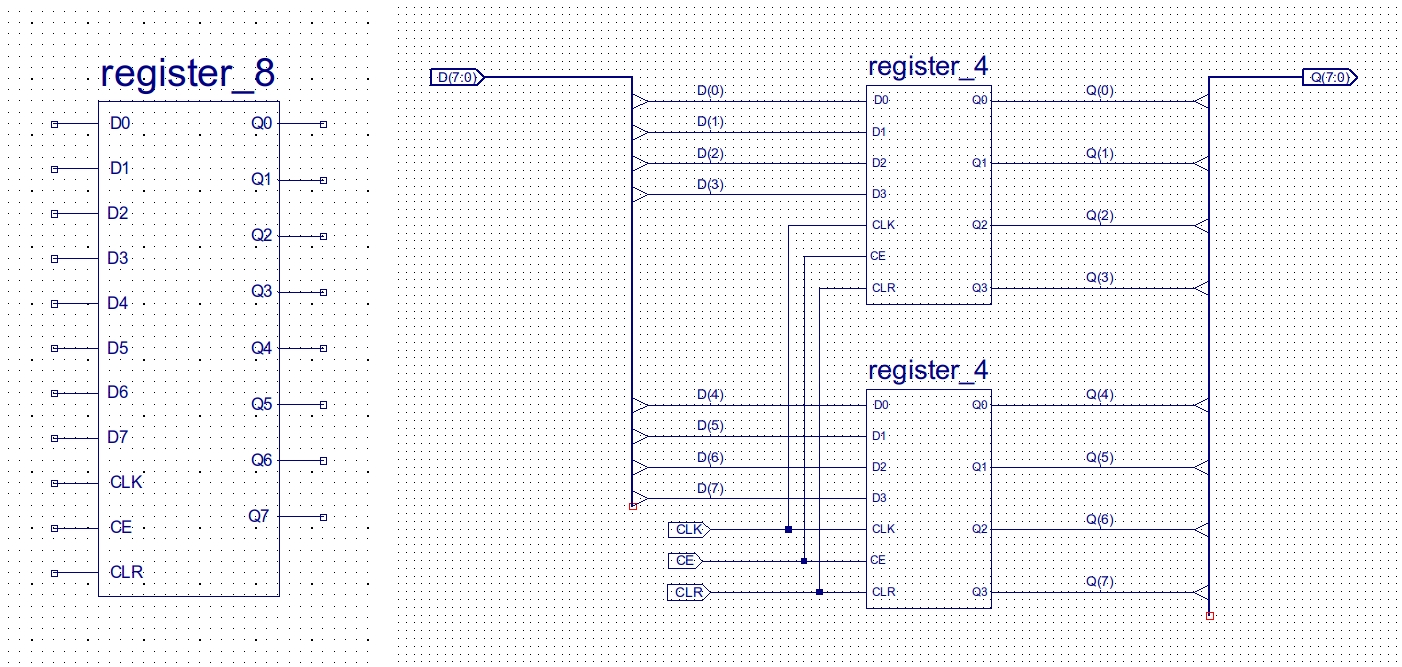
\includegraphics[width=.9\linewidth]{./images/reg8.jpg}
\caption{\label{fig:org474119b}
}
\end{figure}
Accumulator (ACC) : \emph{8} bit register, a general purpose data register, providing data (operand) to be processed by the ALU and used to \textbf{store} any result produced. Note, we can only store one 8 bit value at a time on the processor, other data values will need to be buffered in external memory.
\subsubsection{Interface}
\label{sec:org4e53537}
module pc (\\
d,\\
clk,\\
ce,\\
clr,\\
q\\
);

input [7:0] d     ; \\
input clk         ;   \\
input ce      ; \\
input clr     ; \\
output [7:0] q; \\

\begin{center}
\begin{tabular}{lll}
signal name & type & size\\
\hline
d & input & 8 bits\\
clk & input & 1 bit\\
ce & input & 1 bit\\
clr & input & 1 bit\\
q & output & 8 bits\\
 &  & \\
\hline
\end{tabular}
\end{center}
\subsection{ALU}
\label{sec:org7114248}
\subsubsection{Theory}
\label{sec:orgf20ee77}
\subsubsection{Interface}
\label{sec:org09ca388}
\subsection{MUX}
\label{sec:orge647b52}
\subsubsection{MUX\(_{\text{IR to ALU}}\)}
\label{sec:org7a42dc1}
\subsubsection{MUX\(_{\text{PC to ALU}}\)}
\label{sec:orga5b05aa}
\subsubsection{MUX\(_{\text{Address in RAM}}\)}
\label{sec:org5d38cb4}
\end{document}
